\input{../../../headers/tpheaders.tex}

\cleardoublepage

Ce TP se situe dans la continuité du TP sur la gestion de l'hyperstatisme (S05-TP01-I01).

\section{Mise en position des pièces}

\paragraph{Question 1:} Déterminer la mise en position du bras 3.

\reponse[4]

\section{Solution de spécification}

\paragraph{Question 2:} Proposer une solution de spécification de la pièce 3 ainsi que des pièces utiles à sa mise en position. Pour cela compléter le dessin d'ensemble fourni.

\paragraph{Question 3:} Proposer une solution de spécification des autres pièces du système afin de garantir l'assemblage.

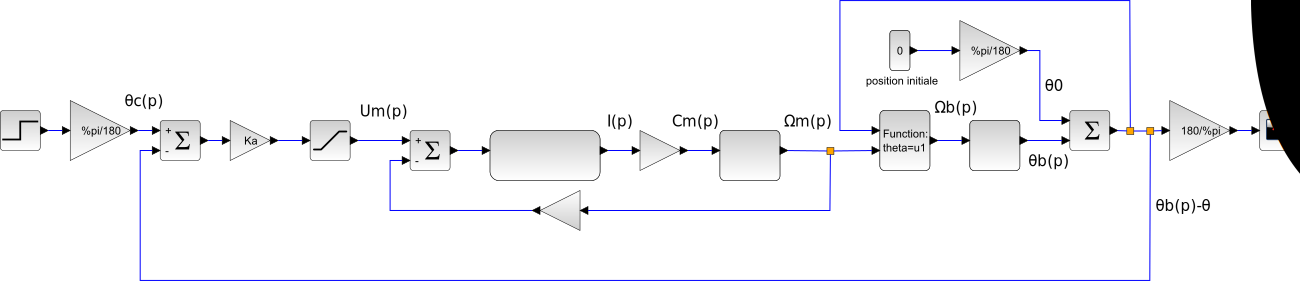
\includepdf{img/Maxpid.pdf}

\end{document}

\pagestyle{correction}\setcounter{section}{0}

\paragraph{Question 1:}
\end{document}